% -*- mode: noweb; noweb-default-code-mode: R-mode; -*-

%\VignetteIndexEntry{Examples: Gaussian process modeling and diagnostics}
%\VignetteKeywords{mlegp}
%\VignettePackage{mlegp}

\section{Examples: Gaussian process fitting and diagnostics}
%\input{cheese}
\subsection{A simple example}
The function {\it mlegp} is used to fit Gaussian processes (GPs) to a vector or matrix of responses observed under the same set of design parameters. Data can be input from within R or read from a text file using the command {\it read.table} (type '?read.table' from within R for more information). The example below shows how to fit multiple Gaussian processes to multiple outputs $z1$ and $z2$ for the design matrix $x$.
Diagnostic plots are obtained using the {\it plot} function, which graphs observed values vs. cross-validated predicted values for each GP. The plot obtained from the code below appears in Figure (\ref{fig:diag1}).

\begin{Schunk}
\begin{Sinput}
> x = -5:5
> z1 = 10 - 5 * x + rnorm(length(x))
> z2 = 7 * sin(x) + rnorm(length(x))
> fitMulti = mlegp(x, cbind(z1, z2))
> plot(fitMulti)
\end{Sinput}
\end{Schunk}
\begin{figure}[htbp]
  \begin{center}
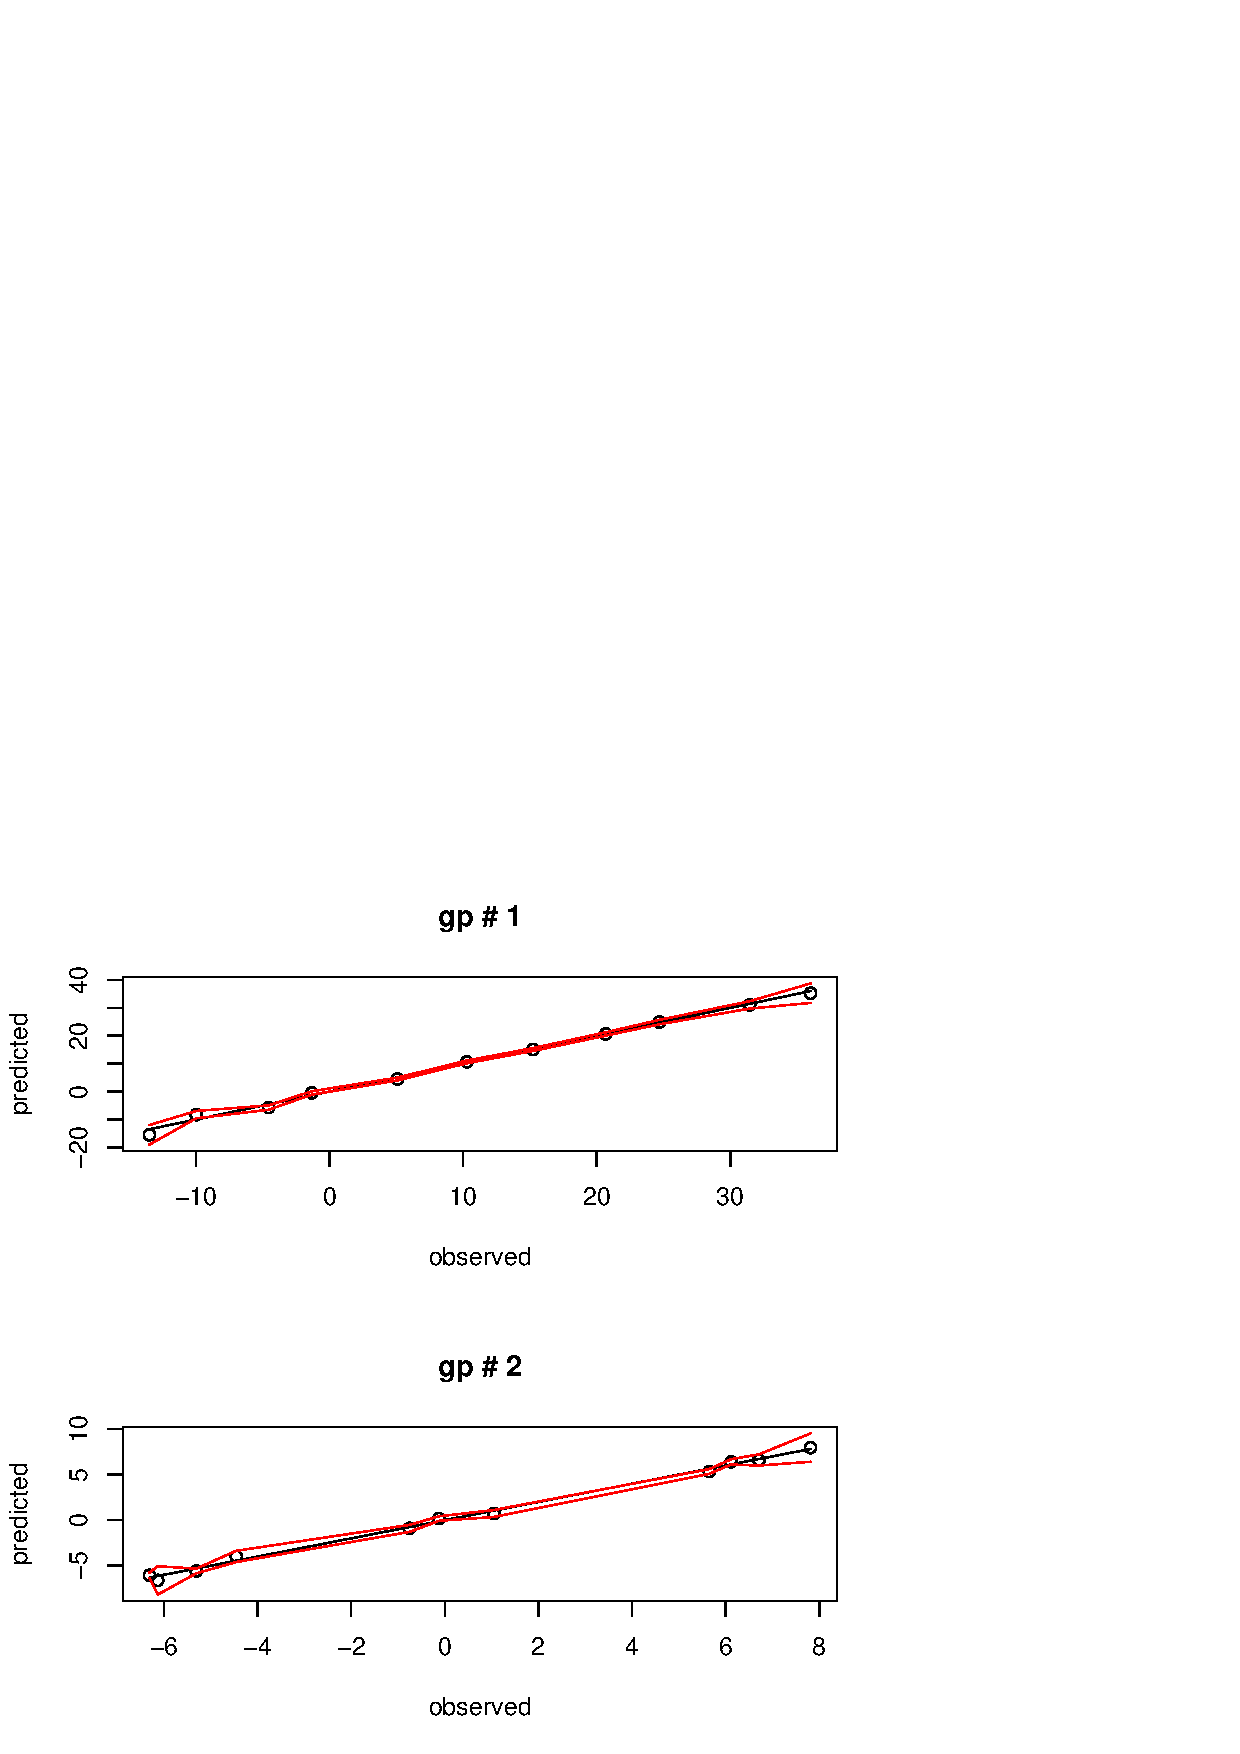
\includegraphics{gp_ex-003}
    \caption{Gaussian process diagnostic plots. Open circles, cross-validated predictions; solid black lines, observed values; solid red lines, confidence bands corresponding to cross-validated predictions $\pm$ standard deviation.}
    \label{fig:diag1}
  \end{center}
\end{figure}

After the GPs are fit, simply typing the name of the object (e.g., $fitMulti$) will return basic summary information. 
\begin{Schunk}
\begin{Sinput}
> fitMulti
\end{Sinput}
\begin{Soutput}
num GPs: 2
Total observations (per GP): 11
Dimensions: 1
\end{Soutput}
\end{Schunk}
We can also access individual Gaussian processes by specifying the index. The code below, for examples, displays summary information for the first Gaussian process, including diagnostic statistics of cross-validated root mean squared error (CV RMSE) and cross-validated root max squared error (CV RMaxSE), where squared error corresponds to the squared difference between cross-validated predictions and observed values.
\begin{Schunk}
\begin{Sinput}
> fitMulti[[1]]
\end{Sinput}
\begin{Soutput}
Total observations = 11
Dimensions = 1

mu = 11.35653
sig2:	183.8340
nugget:	0

Correlation parameters:

       beta a
1 0.1981668 2

Log likelihood = -32.81326

CV RMSE: 0.9680996
CV RMaxSE: 3.978897
\end{Soutput}
\end{Schunk}
\subsection{Heteroscedastic responses and the nugget matrix}
In cases where the responses are heteroscedastic (have non-constant variance), it is possible to specify the diagonal nugget matrix up to a multiplicative constant. Future versions of {\it mlegp} will allow more complicated forms of the nugget matrix; currently, we recommend specifying the nugget matrix based on sample variances for replicate design points (which is easily obtained using the function {\it varPerReps}), or the use of prior information. In the example below, we demonstrate how to fit a Gaussian process with a constant nugget term and a Gaussian process where the diagonal nugget matrix is specified up to a multiplicative constant. First we generate heteroscedastic data, with variance related to the design parameter.   

\begin{Schunk}
\begin{Sinput}
> x = seq(1, 10, by = 0.15)
> z = sin(x) + rnorm(length(x), sd = 0.2 * x)
\end{Sinput}
\end{Schunk}

By default, a nugget term is automatically estimated if there are replicates in the design matrix, and is not estimated otherwise. However, one can estimate a nugget term by specifying an initial scalar value for the \lq nugget\rq\ argument during the call to
{\it mlegp}. This is done in the code below.  

\begin{Schunk}
\begin{Sinput}
> fit1 = mlegp(x, z, nugget = mean((0.2 * x)^2))